\documentclass[a4paper]{article}
\usepackage[dutch]{babel}
\usepackage{amsmath,mathtools,listings,tikz}
\usetikzlibrary{babel}

\author{Benny Aalders}
\title{Sript voor het vinden van de \emph{ggd} en het \emph{kgv} van een lijst met maximaal 255 getallen}
\date{}

\def\pijl{
	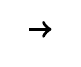
\begin{tikzpicture}[very thick,x=1em,y=1em,baseline={(0,-0.35em)}]
		\draw [->](-0.4,0) -- (0.4,0);
	\end{tikzpicture}
	}
\def\eindpijl{
	
\begin{tikzpicture}[very thick,x=1em,y=1em,baseline={(0,-0.3em)}]
		\draw[<-] (-0.25,0) -- (0.25,0) -- (0.25,0.3); 
	\end{tikzpicture}
	}
\def\dakje{
	
\begin{tikzpicture}[very thick,x=1em,y=1em,baseline={(0,0)}]
		\draw (-0.3,0.3) -- (0,0.7) -- (0.3,0.3);
	\end{tikzpicture}
	}
\def\dh{
	
\begin{tikzpicture}[very thick,x=1em,y=1em,baseline={(0,0)}]
		\filldraw (0,0) -- (0.3,0) -- (0.3,0.3) -- cycle;
	\end{tikzpicture}
	}
\def\sp{\bfseries\textvisiblespace}
\lstset{
	language=[Visual]Basic,
	keywordstyle=\bfseries\underbar,
	commentstyle=\itshape\small,
	keepspaces=true,
%	framexleftmargin=12mm,
	frame=tBlR,
	rulesepcolor=\color[RGB]{204,0,0},
	numbers=left,
	tabsize=2,
	breaklines=true,
	breakatwhitespace=true,
%	showstringspaces=false,
	mathescape=true,
	morekeywords={To,LpWhile,IfEnd,Step,Lbl,Locate,ClrText,Fill},
	escapechar=!,
	captionpos=b,
	literate={->}{\pijl}1 {;}{\eindpijl}1{^}{\dakje}1{;;}{\dh}1
	}
\begin{document}
\maketitle

\noindent Hieronder staat mijn script voor het vinden van de ggd en het kgv. In eerste instantie wilde ik een script schrijven dat zo goed als hetzelfde was als die van Vincent. Dit leek me niet heel erg nuttig. Ik heb daarom een script geschreven dat je misschien van een leerling zou kunnen verwachten dat op een wat hoger niveau zit.

 Zoals ik het nu geschreven heb, vindt het script zowel de ggd als het kgv. Waarschijnlijk zullen leerlingen twee aparte scripts maken. De procedures voor het vinden van de ggd en het kgv lopen niet door elkaar (op het nullen van wat counters na). Hoe leerlingen twee aparte scripts kunnen maken is dus vrij makkelijk af te leiden uit het huidige script. Het script is geschreven voor mijn Casio CFX-9850GC PLUS. 

\lstinputlisting[caption={Script voor het berekenen van de \emph{ggd} en het \emph{kgv}, geschreven in Casio-Basic.}]{GGDKGV-casioBASIC.txt}


\end{document}